% !TEX root=../main.tex
\section{Classical Approach}
\label{sec:classical}

In an effort to better understand the vision problem presented, we first
describe a classical approach to the TurtleBot control problem. Implementation
of the methods described here was done in C++ using the OpenCV
library~\cite{opencv_library}. As described above, we seek to control the
TurtleBot robot through a track outlined with a pair of white ropes. The
commanded control of the robot must only depend on the current image from the
camera mounted on the robot.

Figure~\ref{fig:raw_img} shows an example image from the camera mounted on the
TurtleBot. As seen in this image, the lower quarter of the image is taken up by
the robot itself, effectively providing no useful information to control from.
Based on experimentation, at the constant velocity of 0.3 $m/s$ used for our
experiments, the top section of the image also does not provide any relevant
information for the current control. For these reasons, we first crop out the top
and bottom of the image to produce an image like that seen in 
Figure~\ref{fig:classical_crop}.

The first step in the classical end-to-end control approach is to detect the
ropes in the camera image. As the ropes do not change color, we employ a simple
segmentation method based on color. To segment the white color of the ropes, we
transform the image from RGB color space to HLS (Hue Lightness Saturation)
color space. The color white is found in the HLS space at any values for hue and
saturation with a high value for lightness. Using this knowledge, we create a
mask of the targeted color, white, using a threshold value on the lightness
value of each pixel. The result of this method is a binary mask as seen in
Figure~\ref{fig:classical_thresh}.

The second step of the classical approach is to locate and classify the left
rope and the right rope. In an ideal scenario, such as that depicted in
Figure~\ref{fig:classical_thresh}, this is as simple as detecting the two
largest contours in the binary mask and classifying the left contour as the left
rope and the right contour as the right rope. If no contour is detected on
either side, we declare that particular rope to be out of the field of view of
the camera. Classifying the ropes becomes
ambiguous in scenarios such as that depicted in Figure~\ref{fig:classical_fail}
when the rope is seen lengthwise across the image. This is the major downfall of
an end-to-end approach using only the current camera image. When the robot
approaches a sharp turn or gets into a bad configuration, the camera image can
appear like Figure~\ref{fig:classical_fail} where there is no clear direction
for the robot to follow.

After rope detection and classification, we must compute a steering command. To
compute the desired steering command, we first fit a second order spline to each
of the detected ropes as seen in Figure~\ref{fig:classical_fit}. This spline
fitting serves to smooth out the desired path to follow. We evaluate each spline
at a given height in the image, near the top of the cropped image. We then
average these spline evaluations to get an approximate for our location between
the ropes. We then multiply the error between this average of these spline
evaluations and the center of the image by a proportional gain to get the
desired angular velocity of the TurtleBot.

\begin{figure}
  \centering
  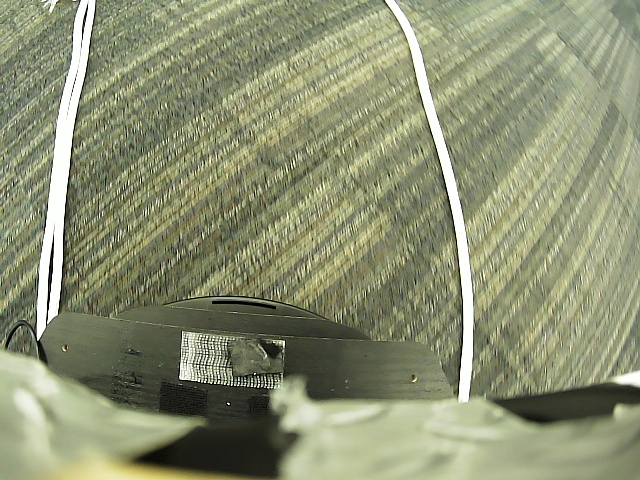
\includegraphics[scale=0.5]{figures/raw_img.png}
  \caption{Example image from the camera mounted on the TurtleBot.}
  \label{fig:raw_img}
\end{figure}

\begin{figure}
  \centering
  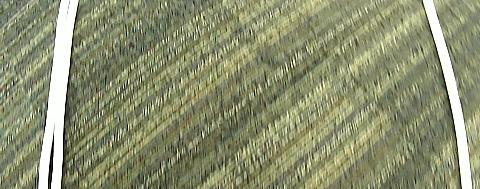
\includegraphics[scale=0.67]{figures/classical_crop.jpg}
  \caption{Cropped image from TurtleBot.}
  \label{fig:classical_crop}
\end{figure}

\begin{figure}
  \centering
  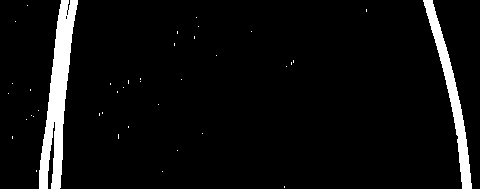
\includegraphics[scale=0.5]{figures/classical_thresh.jpg}
  \caption{TurtleBot image mask after thresholding.}
  \label{fig:classical_thresh}
\end{figure}

\begin{figure}
  \centering
  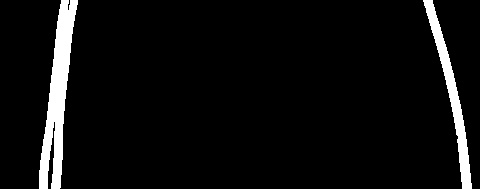
\includegraphics[scale=0.5]{figures/classical_contours.jpg}
  \caption{TurtleBot image mask with only the largest contours.}
  \label{fig:classical_contours}
\end{figure}

\begin{figure}
  \centering
  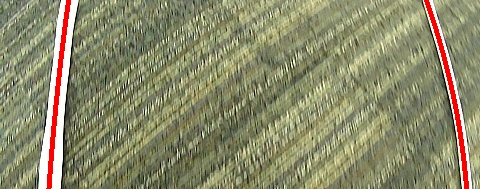
\includegraphics[scale=0.5]{figures/classical_fit.jpg}
  \caption{TurtleBot image with splines fit to largest contours.}
  \label{fig:classical_fit}
\end{figure}

\begin{figure}
  \centering
  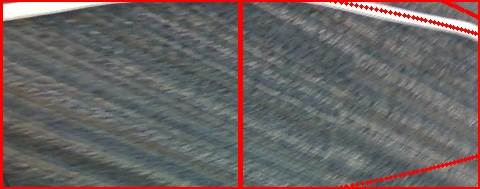
\includegraphics[scale=0.5]{figures/classical_fail.jpg}
  \caption{Example of a failure mode of the classical end-to-end control method.}
  \label{fig:classical_fail}
\end{figure}
